\section{Damping of Betatron Oscillations}\label{sec:4.3}
It is now time to take a look at the so-called radiation damping of the betatron oscillations. I shall give here only an approximate treatment, but using a method which can -- with only a bit of tedious algebra -- be extended to an exact calculation. The exact result is, in any case, obtained more easily by a general theorem that will be discussed in the next section.\\
Let's look first at the vertical betatron oscillations (the notation will be the one used in Part II). I shall approximate the motion by ignoring the variation of $\beta$ with $s$, then I may write (see Section \ref{sec:2.8})
\begin{align}
	z = A \cos(\varphi), && z' = \dfrac{A}{\beta}\sin(\varphi),
\end{align}
where $\varphi$ is $s/\beta$. The amplitude $A$ of the oscillations can be obtained from $z$ and
$z'$ at any instant by
\begin{align}
	A^2 = z^2 + (\beta z')^2
\end{align}
Suppose we are looking at an electron of energy $E_0$ -- which is then oscillating vertically
 about the design orbit. In any element of azimuth $\delta s$ the electron will lose by radiation
 the small amount of energy $\delta E$. Its momentum vector $\bm{p}$ will be changed by $\delta \bm{p}$ and, as was remarked earlier $\delta \bm{p}$ is parallel (and opposite) to $\bm{p}$,so $|\delta \bm{p}| = \delta E/c$. See Fig.~\ref{fig:fig40}(a). The radiation loss does not change either the displacement or the slope of the trajectory; and so the amplitude $A$ is unchanged
by the radiation (there is a small effect due to the fact that the effective focusing forces and, therefore, also $\beta$ are changed with a change of energy but this so-called "adiabatic" damping effect is of second order and can, anyway, be neglected since the energy is not changing on the average when the rf acceleration is also taken into account).

\begin{figure}[!htb]
	\centering
	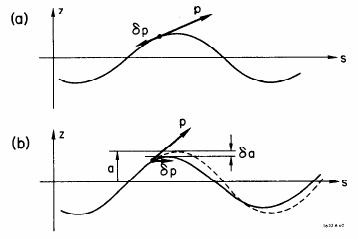
\includegraphics[width=0.8\linewidth]{./Figuras/fig40.jpeg}
	\caption{Effect of an energy change on the vertical betatron oscillations: (a) for radiation loss, (b) for rf acceleration.}
	\label{fig:fig40}
\end{figure}

Notice now, that the effect of the rf accelerating force is quite different. This force is, on the average, parallel to the design orbit. Then the momentum increment $\delta\bm{p}$ received in the azimuthal element $\delta s$ is no longer exactly parallel to $\bm{p}$. See Fig. \ref{fig:fig40}(b). Let's write $p_\perp$, for the component of $\bm{p}$ perpendicular to the design orbit; then, since the angles are small we may write
\begin{align}
	z' = \dfrac{p_\perp}{p}
\end{align}
Again, the accelerating force doesn't change $z$. But now it does change $z'$ which goes over to
\begin{align}
	z' = \dfrac{p_\perp}{p + \delta p} = \dfrac{p_\perp}{p} \left( 1 - \dfrac{\delta p}{p} \right) = z' \left( 1 - \dfrac{\delta p}{p} \right).
\end{align}
The change in z’ is
\begin{align}
	\delta z' = -z' \dfrac{\delta p}{p} = -z' \dfrac{\delta E}{E}.
\end{align}
There is a corresponding change in the amplitude $A$;
\begin{align}
	A \delta A = \beta^2 z' \delta z' = -(\beta z')^2 \dfrac{\delta E}{E}.
\end{align}
Now the phase of the oscillation at the arrival of the electron at the point $s$ is arbitrary
 (and all values between $0$ and $2\pi$ are equally probable) so we should inquire only about the average change in $A$. The average of $(z')^2$ is $A^2/2\beta^2$, so
\begin{align}
	A \mean{\delta A} = - \dfrac{A^2}{2} \dfrac{\delta E}{E_0}.
\end{align}
Suppose we now sum over all the elements of acceleration gain in one revolution. Since all of the $\delta E$ must add up to the radiation loss $U_0$, we find for the change $\Delta A$ that occurs in $A$ during one revolution (due to the rf acceleration):
\begin{align}
	\dfrac{\Delta A}{A} = - \dfrac{U_0}{2 E_0}.
\end{align}
Since $\Delta A$ in each revolution time $T_0$ is proportional to $A$, the motion is exponentially damped -- as $e^{-\alpha_z t}$ . That is,
\begin{align} \label{eq:4.31}
	\dfrac{1}{A} \dfrac{dA}{dt} = \dfrac{\Delta A}{A T_0} = - \dfrac{U_0}{2 E_0 T_0},
\end{align}
so the damping coefficient is
\begin{align}
	\alpha_z = \dfrac{U_0}{2 E_0 T_0} = \dfrac{\mean{P_\gamma}}{2 E_0}.
\end{align}
You can show that an exact calculation -- using the full-blown form for the vertical betatron oscillation -- yields the same result. Notice that the damping rate for the vertical oscillations
 is just $1/2$ the typical rate for the energy oscillations (when $\mathscr{D}$ is small); see Eq.~\eqref{eq:4.20}.\\
It is amusing to notice that the "radiation" damping does not occur in the radiation process, but rather in the process of energy gain from the rf system. One might question the appropriateness of the name "radiation damping". But on second thought, there would be no opportunity for damping by the rf fields if there were not the necessity to compensate for the energy loss by radiation. So the name "radiation damping" is not so bad.\\
Now let’s turn to the radiation effects on the radial betatron oscillations. You might at first,
 think that the radial betatron oscillations would be radiation damped in the, same way as the vertical ones. But there are additional complications so we shall have to treat them as a new problem. One new element arises from the change in the betatron displacement that occurs when there is an energy change. Remember that the total radial displacement $x$ is the sum of two parts: the displacement $x_\epsilon$ of the off-energy closed orbit, plus the betatron displacement $x_\beta$ with respect to the closed orbit,
\begin{align} \label{eq:4.33}
	x = x_\epsilon + x_\beta.
\end{align}
When the energy of an electron changes by $\delta E$, there is a change of $x_\epsilon$ by the
amount, see Eq.~\eqref{eq:2.28},
\begin{align}
	\delta x_\epsilon = \eta \dfrac{\delta E}{E_0}.
\end{align}
But since the position in space of the electron is not changed by a finite momentum impulse,
 the total $x$ does not change, so there must be a compensatory change in $x_\beta$. That is, from Eq.~\eqref{eq:4.33},
\begin{align*}
	\delta x = \delta x_\epsilon + \delta x_\beta = 0,
\end{align*}
from which
\begin{align} \label{eq:4.35}
	\delta x_\beta = -\delta x_\epsilon = -\eta \dfrac{\delta E}{E_0}.
\end{align}
When there is an energy change, the electron doesn't instantaneously move, but the reference
 axis of its oscillations does and the displacement with respect to that axis is therefore changed -- as is illustrated in Fig.~\ref{fig:fig41}.

\begin{figure}[!htb]
	\centering
	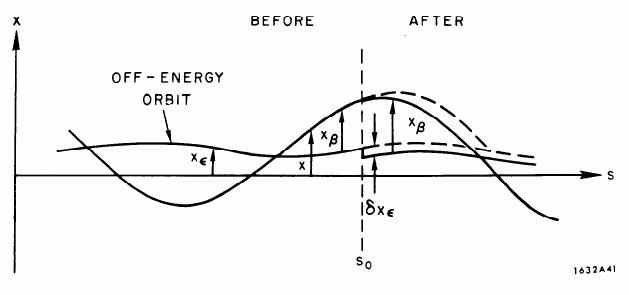
\includegraphics[width=0.8\linewidth]{./Figuras/fig41.jpeg}
	\caption{Effect of a sudden energy change at $s_0$ on the betatron displacement.}
	\label{fig:fig41}
\end{figure}
Something similar occurs for the betatron slope. Corresponding to Eq.~\eqref{eq:4.33} we must have
\begin{align}
	x' = x_\epsilon'+x_\beta'.
\end{align}
Only now, an elementary impulse may change the total $x'$ by some $\delta x'$ so we should
have for the change in the betatron slope
\begin{align}
	\delta x_\beta' = \delta x' - \delta x_\epsilon'.
\end{align}
Taking the derivative $x_\epsilon'$ from Eq.~\eqref{eq:2.28},
\begin{align} \label{eq:4.38}
	\delta x_\beta' = \delta x' - \eta' \dfrac{\delta E}{E_0}.
\end{align}
where $\eta'$ is, of course, $d\eta/ds$. Even if $\delta x'$ were zero, a change in the slope of $x_\epsilon$ the baseline of the oscillations -- would produce a change in the slope of the betatron oscillation.\\
Still an additional complication arises from the curvature of the reference orbit. The positive
 and negative halves of a betatron oscillation occur in equal intervals of $s$, but the electron
 travels a greater path length on the positive swing than on the negative swing - see Eq.~\eqref{eq:3.7}. Although the net effect on the path length is zero, over a complete oscillation, there is, in general, a different amount of energy lost by radiation during the two halves of an oscillation. And the amplitude of the oscillation is thereby affected.\\
Now let's apply these ideas to the radiation loss $\delta E$ in an azimuthal element $\delta s$.
 A precise calculation would proceed from the changes in $x$ and $x'$ found in Eqs. \eqref{eq:4.35} and \eqref{eq:4.38}. In keeping with the approximations made earlier in this
section, however, I am going to make the simplifying assumption that $\eta$ is a constant, so that $\eta' = 0$; and write the variation of $x_\beta$ with $s$ in the same form that I took for $z$; namely,
\begin{align}
	x_\beta = A \cos \varphi; && x_\beta' = \dfrac{A}{\beta} \sin \varphi.
\end{align}
This time we have that
\begin{align}
	A \delta A = x_\beta \delta x_\beta + \beta^2 x_\beta' \delta x_\beta',
\end{align}
and since only $\delta x_\beta$ is different from zero,
\begin{align} \label{eq:4.41}
	A \delta A = - x_\beta \eta \dfrac{\delta E}{E_0}
\end{align}
Again let's take the energy change $\delta E$ as the radiation loss in an azimuthal element $\delta s$. For the $z$-motion we assumed that the electron was always moving with zero radial displacement so the rate of radiation loss was the same (to first order in $z$) as the rate of energy loss on the design orbit. Things are different for the $x$-motion if the magnets have a field gradient. To simplify the discussion here I will restrict consideration to an isomagnetic
 and separated function guide field (see Section \ref{sec:2.2}). In a separated function machine the rate of radiation loss is independent of $x$ -- to first order\footnote{There is only a field gradient in the quadrupoles; where $B$ is proportional to $x$. Since the rate of radiation varies is $B^2$ there is no first order effect.}. I may then take that (for an electron of the nominal energy) the rate of radiation loss $P_\gamma(s)$ does not depend on $x$, but only on $s$.
The energy change in a path element is then
\begin{align}
	\delta E = P_\gamma \dfrac{\Delta \ell}{c}.
\end{align}
Taking for $\Delta \ell$ the expression in \eqref{eq:2.15},
\begin{align}
	\delta E = - P_\gamma \left( 1 + \dfrac{x_\beta}{\rho_s} \right) \dfrac{\Delta s}{c} .
\end{align}
Combining this result with Eq.~\eqref{eq:4.41} we have for the amplitude change,
\begin{align}
	A \delta A = x_\beta \eta P_\gamma \left( 1 + \dfrac{x_\beta}{\rho_s} \right) \dfrac{\Delta s}{c}
\end{align}
Again we are interested only in the expectation value of $\delta A$ -- the average over all
phase angles $\varphi$. The expectation value of $x$ is zero and of $x^2$ is $A^2/2$; we get that
\begin{align}
	\dfrac{\mean{\delta A}}{A} = \dfrac{\eta P_\gamma}{2 \rho_s} \dfrac{\Delta s}{cE_0}
\end{align}
Since I am assuming an isomagnetic guide field wherever $P_\gamma$ is different from zero $\rho = \rho_s = 1/G_0$ and we can easily sum up the effect at each $\Delta s$ to get the change $\Delta A$ in one complete revolution. The sum of all $P_\gamma s/c$ is just the energy loss $U_0$ in one complete turn. So we have for the effect of the radiation
\begin{align}
	\left( \dfrac{\Delta A}{A} \right)_\text{rad} = \dfrac{\eta}{2\rho_0}\dfrac{U_0}{E_0}.
\end{align}
Observe that the sign on the right hand side is positive. There is an increase of the amplitude
 due to the radiation!\\
Fortunately, this is only part of the story. We must also take into account the effect of the rf acceleration. For it however, there is no corresponding "path length" effect. Generally the rf cavities are located in places where $\rho = \infty$ ; but in any case, it is a property of such cavities that the energy gain is (to first order at least) independent of the betatron displacement. The calculation of the contribution from the rf acceleration goes exactly the same as for the vertical oscillations with the result shown in Eq.~\eqref{eq:4.31}. To get the total effect in one revolution we must add the contributions from the radiation loss and from the acceleration to get
\begin{align}
	\dfrac{\Delta A}{A} = - \left(1 - \dfrac{\eta}{\rho_0} \right) \dfrac{U_0}{2 E_0}.
\end{align}
which gives for the damping coefficient $\alpha_x$ of the radial oscillations
\begin{align}\label{eq:4.48}
	\alpha_x = - \left(1 - \dfrac{\eta}{\rho_0} \right) \dfrac{U_0}{2 E_0 T_0}.
\end{align}
A precise calculation for a separated function isomagnetic guide field gives exactly the same result, if we replace $\eta$ by $\mean{\eta}_\text{Mag}$, the mean value of $\eta(s)$ in the magnets. But recalling Eq.~\eqref{eq:3.14}, $\mean{\eta}_\text{Mag} = 2\pi L\alpha$ so
\begin{align} \label{eq:4.49}
	\alpha_x = - \left(1 - \dfrac{\alpha L}{2\pi\rho_0} \right) \dfrac{U_0}{2 E_0 T_0}. && \left(\begin{tabular}{l}
\text{isomag} \\
\text{sep. func.}
\end{tabular}\right)
\end{align}
Provided $\alpha L/2\pi\rho_0$ is less than 1 -- as it usually is -- the damping coefficient
 is positive and the radial oscillations are damped. But there is an "antidamping" effect of the radiation -- the term $\alpha L/2\pi\rho_0$ -- which counteracts somewhat the positive damping from the rf system. So long as the antidamping term is small no harm is done.
If you compare Eq.~\eqref{eq:4.49} with the results of the preceding section you will see that we may also write our result in terms of the parameter $\mathscr{D}$ defined there:
\begin{align}\label{eq:4.50}
	\alpha_x = (1-\mathscr{D}) \dfrac{U_0}{2E_0 T_0}. && (\text{general})
\end{align}
Although we have demonstrated this result only for a special kind of guide field (and with some approximations) Eq.~\eqref{eq:4.50}, it turns out, is exactly -- true for any guide field. That is, if we had in our treatment kept account of the effect of the variation of $\eta$ with $s$ we would have found that in place of $\eta/\rho_0$ in Eq.~\eqref{eq:4.48} we would have the complete expression for $\mathscr{D}$ in Eq.~\eqref{eq:4.17}. More will be said about this interesting "coincidence" in the next section.
